\documentclass[tikz,border=10pt]{standalone}
\begin{document}
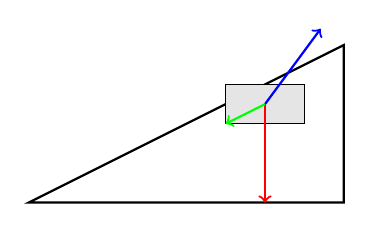
\begin{tikzpicture}[scale=1, auto, every node/.style={scale=0.8}]

% Drawing inclined plane
\draw[thick] (0,0) -- (4,0) -- (4,2) -- cycle;

% Drawing car as a block
\draw[fill=gray!20] (2.5,1) rectangle (3.5,1.5);

% Drawing forces
\draw[thick,->,red] (3,1.25) -- (3,0); % Gravity force
\draw[thick,->,blue] (3,1.25) -- (3.707,2.207); % Normal force
\draw[thick,->,green] (3,1.25) -- (2.5,1); % Friction force

\end{tikzpicture}
\end{document}